\documentclass[a4paper,11pt]{thesis}

% {{{ PACKAGES
% {{{ ENCODAGE ET POLICE
\usepackage[utf8]{inputenc}
\usepackage[T1]{fontenc}
\usepackage[french]{babel}
\usepackage{eurosym}
% }}}

% {{{ FIGURES
\usepackage{graphicx}
\usepackage{subfig}
% }}}

% {{{ INSERTION DE CODE
\usepackage{moreverb}
% }}}

% {{{ INSERTION DE PDF
\usepackage{pdfpages}
% }}}

% {{{ RÉDUCTION DES MARGES
%\usepackage{fullpage}
%\usepackage[top=2.5cm, bottom=2.5cm, left=3.5cm, right=3.5cm]{geometry}
% }}}

% {{{ MATHÉMATIQUES
\usepackage{amsmath}
\usepackage{amsthm}
\usepackage{bbm}
\usepackage{amssymb}
\usepackage{stmaryrd}
% }}}

% {{{ GRAPHES
\usepackage{tikz}
\usepackage{pgf}
\usetikzlibrary{arrows,automata,shapes}
% }}}

% {{{ RESEAUX DE pETRI
\usetikzlibrary{petri}
% }}}

% {{{ ARBRES
\usetikzlibrary{trees}
% }}}

% {{{ DIAGRAMME DE GANTT
\usepackage{pgfgantt}
% }}}

% {{{ ALGORITHMES
\usepackage{algorithm}
\usepackage[noend]{algpseudocode}
%\usepackage{algorithmic}
%\usepackage{algorithmicx}
% }}}
% }}}

% {{{ NEWTHEOREM
% {{{ THÉORÈMES, lEMMES -- NUMÉROTATION PERSONNALISÉE
\theoremstyle{plain}
\newtheorem{thrm}{Théorème}[section]
\newtheorem{lemm}{Lemme}[subsection]
\newtheorem{corol}{Corollaire}[section]
% }}}

% {{{ THÉORÈMES, lEMMES -- NUMÉROTATION CLASSIQUE
\newtheorem{nthrm}{Théorème}
\newtheorem{nlemm}{Lemme}
\newtheorem{ncorol}{Corollaire}
\newtheorem{npb}{Problème}
% }}}

% {{{ THÉORÈMES, lEMMES -- NON NUMÉROTÉS
\newtheorem*{thrm*}{Théorème}
\newtheorem*{lemm*}{Lemme}
\newtheorem*{corol*}{Corollaire}
% }}}

% {{{ DÉFINITIONS, pROPRIÉTÉS -- NUMÉROTATION PERSONNALISÉE
\theoremstyle{definition}
\newtheorem{df}{Définition}[subsection]
\newtheorem{prop}{Propriété}[subsection]
\newtheorem{conj}{Conjecture}[subsection]
% }}}

% {{{ DÉFINITIONS, pROPRIÉTÉS -- NUMÉROTATION CLASSIQUE
\newtheorem{ndf}{Définition}
\newtheorem{nprop}{Propriété}
\newtheorem{nconj}{Conjecture}
% }}}

% {{{ DÉFINITIONS, pROPRIÉTÉS -- NON NUMÉROTÉS
\newtheorem*{df*}{Définition}
\newtheorem*{prop*}{Propriété}
\newtheorem*{conj*}{Conjecture}
% }}}

% {{{ AUTRES -- NUMÉROTATION PERSONNALISÉE
\theoremstyle{remark}
\newtheorem{nota}{Note}[subsubsection]
\newtheorem{pr}{Proposition}[subsection]
\newtheorem{rmq}{Remarque}[subsubsection]
% }}}

% {{{ AUTRES -- NUMÉROTATION CLASSIQUE
\newtheorem{nnota}{Note}
\newtheorem{npr}{Proposition}
\newtheorem{nrmq}{Remarque}
% }}}

% {{{ AUTRES -- NON NUMÉROTÉS
\newtheorem*{nota*}{Note}
\newtheorem*{pr*}{Proposition}
\newtheorem*{rmq*}{Remarque}
% }}}

% {{{ EXEMPLES
\newtheorem*{ex}{Exemple}
\newtheorem*{exo}{Exercice}
\newtheorem*{rappel}{Rappel}
% }}}
% }}}

% {{{ OPÉRATEURS MATHÉMATIQUES
\DeclareMathOperator{\poly}{\textbf{poly}}
\DeclareMathOperator{\gap}{\mbox{gap}}
\DeclareMathOperator{\Bg}{\mbox{Big}}
\DeclareMathOperator{\Sml}{\mbox{Sml}}
\DeclareMathOperator{\Diff}{\mbox{Diff}}
\DeclareMathOperator{\card}{\mbox{Card}}
\DeclareMathOperator{\Obj}{\mbox{Obj}}
\DeclareMathOperator{\concat}{\bullet}
\DeclareMathOperator{\sig}{\mbox{Sig}}
\DeclareMathOperator{\ver}{\mbox{Ver}}
\DeclareMathOperator{\dist}{\mbox{dist}}
\DeclareMathOperator{\bw}{\mbox{branchwidth}}
\DeclareMathOperator{\tw}{\mbox{tw}}
\DeclareMathOperator{\lm}{\leq_m}
\DeclareMathOperator{\lc}{\leq_c}
\DeclareMathOperator{\lex}{\mbox{lex}}
\DeclareMathOperator{\ord}{\mbox{ord}}
% }}}

% {{{ MACCROS
% {{{ MACROS DIVERSES
\newcommand{\npc}{$NP-$complet}
\newcommand{\npd}{$NP-$difficile}
\newcommand{\la}{largeur arborescente}
\newcommand{\legendre}[2]{\left ( \frac{#1}{#2} \right )}
\newcommand{\wqo}[0]{\emph{well-quasi-ordered}}
\newcommand{\Tau}[0]{\mathcal{T} = (T, \{X_t : t \in T\})}
\newcommand{\Taug}[0]{\mathcal{T}_G = (T, \{X_t : t \in T\})}
\newcommand{\Taustar}[0]{\mathcal{T}^* = (T, \{X_t : t \in T\})}
\newcommand{\Taugstar}[0]{\mathcal{T}_G^* = (T, \{X_t : t \in T\})}
\newcommand{\pdsol}[1]{(X_{#1}^0, X_{#1}^1, X_{#1}^2, M_{#1})}
% }}}
                
% {{{ NOM DE PROBLEMES
\newcommand{\hcycle}{\textsc{HAMILTONIAN CYCLE} }
\newcommand{\phcycle}[1]{\textsc{HAMILTONIAN CYCLE }paramétré par \textsc{#1} }
\newcommand{\vcover}{\textsc{VERTEX COVER} }
\newcommand{\twidth}{\textsc{TREE WIDTH} }
\newcommand{\wiset}{\textsc{WEIGHTED INDEPENDANT SET} }
\newcommand{\fvset}{\textsc{FEEDBACK VERTEX SET} }
\newcommand{\kvcover}{\textsc{K-Vertex Cover} }
\newcommand{\oct}{\textrm{\textsc{Odd Cycle Transversal}} }
\newcommand{\dlp}{\textrm{\textsc{Discrete Logarithm Problem}} }
\newcommand{\ecdlp}{\textrm{\textsc{Elliptic Curve Discrete Logarithm Problem}} }

% }}}

% {{{ MISE EN PAGE

\newcommand{\dfpbi}[3]{
    \begin{npb}[#1]
        \begin{itemize}
            \itemindent 10mm
            \item[\textbf{Données :}] #2
            \item[\textbf{Problème :}] #3
        \end{itemize}
    \end{npb}
}

\newcommand{\dfpb}[3]{
    \begin{npb}[#1]
        \begin{itemize}
            \itemindent 10mm
            \item[\textbf{Données :}] #2
            \item[\textbf{Question :}] #3
        \end{itemize}
    \end{npb}
}

\newcommand{\dfpbp}[4]{
    \begin{npb}[#1]
        \begin{itemize}
            \itemindent 10mm
            \item[\textbf{Données :}] #2
            \item[\textbf{Paramètre :}] #4
            \item[\textbf{Question :}] #3
        \end{itemize}
    \end{npb}
}
% }}}

% }}}
    
% {{{ TIKZ
%%% {{{ STYLE
\tikzstyle{edge}=[
	-,
	draw=black
]

\tikzstyle{sized}=[
    minimum width=9mm
]

\tikzstyle{tvertex}=[
	node distance=15mm,
    inner sep = 1mm
]

\tikzstyle{tvert}=[
	node distance=5mm,
    inner sep=1mm
]

\tikzstyle{tmvertex}=[
    tvertex,
    sized
]

\tikzstyle{tmvert}=[
    tvert,
    sized
]

\tikzstyle{mvertex}=[
    tmvertex,
	circle,
	draw=black,
	fill=black!50
]

\tikzstyle{mvert}=[
    tmvert,
	circle,
	draw=black,
	fill=black!50
]

\tikzstyle{vertex}=[
    tvertex,
	circle,
	draw=black,
	fill=black!50
]

\tikzstyle{vert}=[
    tvert,
	circle,
	draw=black,
	fill=black!50
]

\tikzstyle{treedec}=[
	vertex,
	node distance=15mm,
	draw=red,
	fill=red!50
]

\tikzstyle{treeedge}=[
	edge,
	draw=red
]

\tikzstyle{giedge}=[
	edge,
	draw=blue
]

\tikzstyle{bounding}=[
	thick, %ultra
	%dash pattern=on 1mm off 1mm,
	densely dotted,
	fill=blue!10,
	draw=blue!70
]

\tikzstyle{patate}=[
    rounded corners=5pt,
    draw=black,
    fill=black!50,
    text width=12mm,
    text centered
]

\tikzstyle{patatoid}=[
    ellipse,
    node distance=10mm,
    draw=black
]
%%% }}}

% {{{ DESSINS
\newcommand{\base}[4]{
    \draw[->] (0,0) to (0, #1);
    \draw[->] (0,0) to (#2, 0);
    
    \node at (0, #1+2) {#3};
    \node at (#2 + 2, -2) {#4};
}
% }}}
%}}}


\pagenumbering{roman}
\pagestyle{fancyplain}
\thispagestyle{empty}
\noindent
\begin{center}
\large{\texttt{Académie de Montpellier}}\\
\Large{\texttt{Université Montpellier II}}\\
\large{\texttt{Sciences et Techniques du Languedoc}}\\
\end{center}

\vspace{1cm}

\begin{center}
\Huge{\textbf{\'{E}TUDE BIBLIOGRAPHIQUE DE\\}}
 \vspace{1.0cm}
\Huge{\textbf{MASTER M2}}
\normalsize
\begin{center}
\vspace{1.0cm}

effectué au Laboratoire d'Informatique de Robotique\\
et de Micro-électronique de Montpellier
\end{center}

\vspace{2mm}
%\Large{\textbf{prÈnom NOM}}

\vspace{0.1cm}
\normalsize

\vspace{3mm}

\large{Spécialité} : \textbf{MOCA}\\
%\Large{Formation Doctorale} : \textbf{Informatique}\\
%\large{{\'E}cole Doctorale} : \textbf{Information, Structures, SystËmes}
\vspace{1.0cm}

\LARGE{\textbf{Complexité et algorithmes d'approximation pour des problèmes d'ordonnancement d'intervalles
avec optimisation de la défragmentation}}
\vspace{2mm}

\begin{center}
  par \textbf{Guillerme DUVILLIÉ}
\end{center}

\vspace{2mm}



\vspace{4cm}

Date de rendu : \textbf{}

\vspace{0.5cm}

Sous la direction de \textbf{Marin BOUGERET, Rodolphe GIROUDEAU et Denis TRYSTRAM}

\vspace{5mm}




\end{center}
\newpage
\tableofcontents
\newpage

\pagenumbering{arabic}


\author{}
\title{}
\location{Montpellier}\blurb{}
\makeatother
\title{Devoir à rendre}
\author{Guillerme DUVILLIE}
\location{Montpellier}
\blurb{
    Université Montpellier II\\
    Master Informatique Modélisation, Optimisation Combinatoire et Algorithmique \\[1em]
    Matière : Complexité paramétrée\\
    Encadrant : Christophe PAUL
}

% Info page_garde
% A REMPLIR
%


\begin{document}

\maketitle
\newpage

% content.tex
% includes all necessary files

%\maketitle
\tableofcontents

\clearpage

% {{{ INTRO
Tout au long de ces notes de cours, nous nous intéresserons au problème du cycle Hamiltonien. 

%% {{{ PRESENTATION DU PLAN
Au cours de la première partie nous démontrerons la $NP-$complétude de \hcycle puis nous
détaillerons des bornes relatives au noyau de ce problème. Dans une seconde partie, nous développerons le
principe de décomposition arborescente et nous détaillerons la notion de largeur arborescente
associée. Cette valeur possède une grande importance dans le monde de la complexité paramétrée
puisqu'elle a permis d'introduire de nouvelles paramétrisations conduisant à des algorithmes FPT
pour des problèmes tels que \wiset ou \hcycle, basés sur la programmation dynamique. La partie
suivante développera en détail un de ces algorithmes sur le problème \hcycle. Enfin nous
présenterons les idées se trouvant derrière les algorithmes de programmation dynamiques utilisé pour
la résolution des problèmes tels que \wiset ou \fvset. 
%% }}}
% }}}


\chapter{Autour de \hcycle}
\label{about_hcycle}
% {{{ RAPPEL SUR LE CYCLE HAMILTONIEN
%% {{{ CYCLE HAMILTONIEN DEFINITION DU PROBLEME
Avant toute chose, définissons de manière formelle le problème sur lequel nous allons travailler.

\dfpb{\hcycle}{$G(V, E)$, un graphe non orienté}{Existe-t-il un chemin $H_G$ de $G$, tel
que tous les sommets de $G$ sont visités par $H$ une seule fois et revenant à son point de départ ?}
%% }}}

%% {{{ NP-COMPLETUDE
\section{$NP-$complétude}
\label{hcycle_npc}
\begin{nthrm}
    Le problème \hcycle est \npc
\end{nthrm}

\begin{proof}
    La preuve sera menée en tois parties. Dans un premier temps, nous décrirons une
    réduction de \vcover à ce problème, puis nous démontrerons qu'une solution existe pour \vcover
    si et seulement si le graphe contruit admet un cycle hamiltonien. Enfin nous clotûrerons cette
    preuve par la preuve que cette réduction se fait en temps polynomial.

    Définissons dans un premier temps le problème \vcover que nous allons utiliser.

    \dfpb{\vcover}{$G(V, E)$ un graphe non orienté et $k$ un entier}{Existe-t-il un ensemble $VC$ de
        sommets de $V$ de taille $k$ tel que toute arête de $E$ est adjacente à au moins un sommet
    de $VC$ ?}

    Ce problème a été démontré \npc~\cite{karp}, dans ce même article Karp démontre aussi
    la $NP-$complétude de \hcycle. %Décrire rapidement la technique utilisée par Karp
    La technique de réduction que nous utilisons consiste à remplacer les
    arêtes du graphe de départ $G$, pour lequel une couverture est cherchée, par un motif
    particulier dans le graphe d'arrivée $G'$, pour lequel nous cherchons un cycle hamiltonien.
    Il existe trois façons de parcourir ce motif de façon à ce que tous les sommets ne soient
    visités qu'une seule fois, correspondant à chacune des trois façons de couvrir l'arête $(uv)$
    ainsi remplacée. Donc pour une arête $(uv) \in E$, le chemin
    hamiltonien décrit à la figure~\ref{motif_u} représente le cas où $u$ appartient au \vcover de
    taille $k$, celui de la figure~\ref{motif_v} représente le cas où $v$ appartient au \vcover de
    taille $k$ et enfin la figure~\ref{motif_uv} représente le cas où $u$ et $v$ appartiennent tous
    deux au \vcover de taille $k$.

    % {{{ MOTIFS DE REMPLACEMENT
    \begin{figure}
        \begin{center}
            \begin{tikzpicture}
                \node[vertex] (u1) {$u_1$};
\node[vertex, below=of u1] (v1) {$v_1$};

\foreach \x [evaluate=\x as \y using (\x - 1)] in {2,...,6} {
    \node[vertex, right=of u\y] (u\x)  {$u_{\x}$};
    \node[vertex, right=of v\y] (v\x)  {$v_{\x}$};
    \draw[edge] (u\y) to (u\x);
    \draw[edge] (v\y) to (v\x);
}

\draw[edge] (u1) to (v3);
\draw[edge] (v1) to (u3);
\draw[edge] (u4) to (v6);
\draw[edge] (v4) to (u6);


            \end{tikzpicture}
            \caption{Motif de remplacement d'une arête}
            \label{motif_npc}
        \end{center}
    \end{figure}

    \begin{figure}
        \begin{center}
            \begin{tikzpicture}
                \input{src/figures/motif_hcycle.tex}

%\foreach \x [evaluate=\x as \y using (\x + 1)] in {1, 2, 4, 5} {
%    \draw[draw=red, very thick] (u\x) to (u\y);
%    \draw[draw=red, very thick] (v\x) to (v\y);
%}

\draw[draw=red, line width=2pt] (u1) to (u2);
\draw[draw=red, line width=2pt] (u2) to (u3);
\draw[draw=red, line width=2pt] (u3) to (v1);
\draw[draw=red, line width=2pt] (v1) to (v2);
\draw[draw=red, line width=2pt] (v2) to (v3);
\draw[draw=red, line width=2pt] (v3) to (v4);
\draw[draw=red, line width=2pt] (v4) to (v5);
\draw[draw=red, line width=2pt] (v5) to (v6);
\draw[draw=red, line width=2pt] (v6) to (u4);
\draw[draw=red, line width=2pt] (u4) to (u5);
\draw[draw=red, line width=2pt] (u5) to (u6);

            \end{tikzpicture}
            \caption{Cas 1 : $u$ appartient au \vcover}
            \label{motif_u}
        \end{center}
    \end{figure}

    \begin{figure}
        \begin{center}
            \begin{tikzpicture}
                \input{src/figures/motif_hcycle.tex}

%\foreach \x [evaluate=\x as \y using (\x + 1)] in {1, 2, 4, 5} {
%    \draw[draw=red, very thick] (u\x) to (u\y);
%    \draw[draw=red, very thick] (v\x) to (v\y);
%}

\draw[draw=red, line width=2pt] (v1) to (v2);
\draw[draw=red, line width=2pt] (v2) to (v3);
\draw[draw=red, line width=2pt] (v3) to (u1);
\draw[draw=red, line width=2pt] (u1) to (u2);
\draw[draw=red, line width=2pt] (u2) to (u3);
\draw[draw=red, line width=2pt] (u3) to (u4);
\draw[draw=red, line width=2pt] (u4) to (u5);
\draw[draw=red, line width=2pt] (u5) to (u6);
\draw[draw=red, line width=2pt] (u6) to (v4);
\draw[draw=red, line width=2pt] (v4) to (v5);
\draw[draw=red, line width=2pt] (v5) to (v6);

            \end{tikzpicture}
            \caption{Cas 2 : $v$ appartient au \vcover}
            \label{motif_v}
        \end{center}
    \end{figure}

    \begin{figure}
        \begin{center}
            \begin{tikzpicture}
                \input{src/figures/motif_hcycle.tex}

%\foreach \x [evaluate=\x as \y using (\x + 1)] in {1, 2, 4, 5} {
%    \draw[draw=red, very thick] (u\x) to (u\y);
%    \draw[draw=red, very thick] (v\x) to (v\y);
%}

\draw[draw=red, line width=2pt] (u1) to (u2);
\draw[draw=red, line width=2pt] (u2) to (u3);
\draw[draw=red, line width=2pt] (u3) to (u4);
\draw[draw=red, line width=2pt] (u4) to (u5);
\draw[draw=red, line width=2pt] (u5) to (u6);

\draw[draw=red, line width=2pt] (v1) to (v2);
\draw[draw=red, line width=2pt] (v2) to (v3);
\draw[draw=red, line width=2pt] (v3) to (v4);
\draw[draw=red, line width=2pt] (v4) to (v5);
\draw[draw=red, line width=2pt] (v5) to (v6);

            \end{tikzpicture}
            \caption{Cas 3 : $u$ et $v$ appartiennent au \vcover}
            \label{motif_uv}
        \end{center}
    \end{figure}
    % }}}

    Il s'agit maintenant de relier les motifs entre eux, pour ce faire considérons deux arêtes
    $(uv)$ et $(uw)$ de $E$ adjacentes toutes deux au somet $u$. Chacune de ces arêtes est remplacée
    par le motif présenté précédemment, appelons $U_v$ l'ensemble des sommets $\{u_1, u_2, \dots,
    u_6\}$ du motif correspondant à l'arête $(uv)$ et $U_w$ l'ensemble des sommets $\{u_1, u_2,
    \dots, u_6\}$ du motif correspondant à l'arête $(uw)$. Dans la construction finale, $U_v$ et
    $U_w$ sont reliés entre eux par une arête, comme présenté figure~\ref{hcycle_couple}. Et l'on
    fait de même pour tous les sommets et arêtes de $G'$. Chaque sommet $v$ de $G$ est alors représenté
    par une chaine dans $G'$ composée de $6*d(v)$ sommets.

    Pour illustrer la transformation, considérons le graphe $G = (V, E)$ dont une représentation est
    donnée à la figure~\ref{hcycle_graphe_g}. La figure~\ref{hcycle_graphe_gprime} représente le
    graphe obtenu après transformation des arêtes. On peut ainsi se rendre compte qu'il existe un
    \vcover de taille $k$ si et seulement si il existe $k$ chemins partant du côté gauche et
    arrivant du côté droit passant par l'ensemble des sommets du graphe $G'$.

    Pour arriver à une recherche de \hcycle dans le graphe $G'$ correspondant à un \vcover de taille
    $k$, il suffit de rajouter $k$ sommets $s_1, s_2, \dots, s_k$ reliant le côté droit au côté
    gauche, de sorte qu'une fois arrivé au bout de la chaîne représentant un sommet, il est possible
    de retourner du côté gauche sur une nouvelle chaîne représentant un autre sommet.

    La dernière phase de la transformation, pour un \vcover de taille $2$ est détaillée
    figure~\ref{hcycle_last}, les sommets $1_{deb}$ et $1_{fin}$ désignant respectivement le premier
    et le dernier n\oe ud de la chaîne représentant le sommet $1$. 

    La recherche d'un vetex cover de taille $k$ dans $G$ nous amène donc alors à al recherche d'un
    chemin hamiltonien dans le graphe $G'$ dont une représentation est donnée à la
    figure~\ref{hcycle_finish}.

    % {{{ TRANSFORMATION
    \begin{figure}
        \begin{center}
            \begin{tikzpicture}[scale=0.8, every node/.style={transform shape}]
                \node[tmvert] (u0) {$U$};
\node[tmvert, below=of u0] (tp0) {};
\node[tmvert, below=of tp0] (v0) {$V$};
\node[tmvert, below=of v0] (tp1) {};
\node[tmvert, below=of tp1] (w0) {$W$};

\node[mvert, right=of u0] (u1) {$u_1$};
\node[mvert, right=of v0] (v1) {$v_1$};

\foreach \x [evaluate=\x as \y using (\x - 1)] in {2,...,6} {
    \node[mvert, right=of u\y] (u\x)  {$u_{\x}$};
    \node[mvert, right=of v\y] (v\x)  {$v_{\x}$};
    \draw[edge] (u\y) to (u\x);
    \draw[edge] (v\y) to (v\x);
}

\draw[edge] (u1) to (v3);
\draw[edge] (v1) to (u3);
\draw[edge] (u4) to (v6);
\draw[edge] (v4) to (u6);

\node[mvert, right=of u6] (uw1) {$u'_{1}$};
\node[tmvert, below=of v6] (t2) {};
\node[tmvert, below=of t2] (t3) {};
\node[mvert, right=of t3] (w1) {$w_1$};

\draw[edge] (u6) to (uw1);

\foreach \x [evaluate=\x as \y using (\x - 1)] in {2,...,6} {
    \node[mvert, right=of uw\y] (uw\x)  {$u'_{\x}$};
    \node[mvert, right=of w\y] (w\x)  {$w_{\x}$};
    \draw[edge] (uw\y) to (uw\x);
    \draw[edge] (w\y) to (w\x);
}

\draw[edge] (uw1) to (w3);
\draw[edge] (w1) to (uw3);
\draw[edge] (uw4) to (w6);
\draw[edge] (w4) to (uw6);

\draw[edge] (u0) to (u1);
\draw[edge] (v0) to (v1);
\draw[edge] (w0) to (w1);

            \end{tikzpicture}
            \caption{Liaison de deux motifs représentant deux arêtes adjacentes à un même sommet}
            \label{hcycle_couple}
        \end{center}
    \end{figure}

    \begin{figure}
        \begin{center}
            \begin{tikzpicture}
                \node[vertex] (1) {$1$};
\node[vertex, below=of 1] (2) {$2$};
\node[vertex, below left=of 2] (3) {$3$};
\node[vertex, below right=of 2] (4) {$4$};

\draw[edge, very thick, violet] (1) to (2);
\draw[edge, very thick, green] (2) to (3);
\draw[edge, very thick, orange] (2) to (4);
\draw[edge, very thick, blue] (3) to (4);


            \end{tikzpicture}
            \caption{Exemple de transformation : le graphe $G$}
            \label{hcycle_graphe_g}
        \end{center}
    \end{figure}

    \begin{figure}
        \begin{center}
            \begin{tikzpicture}[scale=0.6, every node/.style={transform shape}, tmp/.style={inner
                    sep=0mm, node distance=3mm}]
                \foreach \x/\y in {2/1, 4/2, 6/3, 8/4}{
    \node[tvert] at (0, \x) (\y) {$\y$};
}

\foreach \w in {0.5}{
    \foreach \x/\y/\col in {1/2/violet, 2/3/green, 3/4/blue, 4/2/orange}{
        \pgfmathparse{int(30*\w + 1)}
        \node[tvert] at (\pgfmathresult, 2*\x) (f\x) {$\x$};
        \draw[edge] (\x) to (f\x);

        \foreach \z in {1, 2, 3, 4, 5, 6}{
            \pgfmathparse{(\x-1)*(7*\w)+1 + (\z*\w)}
            \node[tmp,\col] at (\pgfmathresult, \x*2) (\x\y\z) {$\bullet$};
            \node[tmp,\col] at (\pgfmathresult, \y*2) (\y\x\z) {$\bullet$};
        }

        \foreach \z [evaluate=\z as \a using \z -1] in {2, 3, 4, 5, 6}{
            \draw[edge, \col] (\x\y\a) to (\x\y\z);
            \draw[edge, \col] (\y\x\a) to (\y\x\z);
        }

        \draw[edge,\col] (\x\y1) to (\y\x3);
        \draw[edge,\col] (\x\y3) to (\y\x1);
        \draw[edge,\col] (\x\y4) to (\y\x6);
        \draw[edge,\col] (\x\y6) to (\y\x4);
    }
}

            \end{tikzpicture}
            \caption{Exemple de transformation : le graphe $G'$ obtenu après transformation de $G$}
            \label{hcycle_graphe_gprime}
        \end{center}
    \end{figure}

    \begin{figure}
        \begin{center}
            \begin{tikzpicture}[scale=2, tmp/.style={vertex, minimum size=10mm}]
                \node[tmp] at (3, 3.5) (s1) {$s_1$};
\node[tmp] at (3, 1.5) (s2) {$s_2$};

\foreach \y in {1, 2, 3, 4}{
    \foreach \x/\lab in {0/fin, 6/deb}{
        \node[tmp] at (\x, \y) (\lab\y) {$\y_{\lab}$};
        \draw[edge] (\lab\y) to (s1);
        \draw[edge] (\lab\y) to (s2);
    }
}


            \end{tikzpicture}
            \caption{Exemple de transformation : la dernière phase}
            \label{hcycle_last}
        \end{center}
    \end{figure}

    \begin{figure}
        \begin{center}
            \begin{tikzpicture}[scale=0.6, every node/.style={transform shape}, tmp/.style={inner
                    sep=0mm, node distance=3mm}]
                \foreach \x/\y in {2/1, 4/2, 6/3, 8/4}{
    \node[tvert] at (0, \x) (\y) {$\y$};
}

\foreach \w in {0.5}{
    \pgfmathparse{int(30*\w + 1)}
    \node[vert] at (\pgfmathresult/2, 12) (s1) {$s_1$};
    \node[vert] at (\pgfmathresult/2, -2) (s2) {$s_2$};

    \node[tvert] at (-2, 0) (t1s2) {};
    \node[tvert] at (\pgfmathresult + 2, 0) (t2s2) {};
    \node[tvert] at (-2, 10) (t1s1) {};
    \node[tvert] at (\pgfmathresult + 2, 10) (t2s1) {};

    \draw[edge] (s1) to[out=180, in=90] (t1s1);
    \draw[edge] (s1) to[out=0, in=90] (t2s1);
    \draw[edge] (s2) to[out=180, in=270] (t1s2);
    \draw[edge] (s2) to[out=0, in=270] (t2s2);

    \foreach \x/\y/\col in {1/2/violet, 2/3/green, 3/4/blue, 4/2/orange}{
        \node[tvert] at (\pgfmathresult, 2*\x) (f\x) {$\x$};
        \draw[edge] (\x) to (f\x);

        \foreach \z in {1, 2, 3, 4, 5, 6}{
            \pgfmathparse{(\x-1)*(7*\w)+1 + (\z*\w)}
            \node[tmp,\col] at (\pgfmathresult, \x*2) (\x\y\z) {$\bullet$};
            \node[tmp,\col] at (\pgfmathresult, \y*2) (\y\x\z) {$\bullet$};
        }

        \foreach \z [evaluate=\z as \a using \z -1] in {2, 3, 4, 5, 6}{
            \draw[edge, \col] (\x\y\a) to (\x\y\z);
            \draw[edge, \col] (\y\x\a) to (\y\x\z);
        }

        \draw[edge,\col] (\x\y1) to (\y\x3);
        \draw[edge,\col] (\x\y3) to (\y\x1);
        \draw[edge,\col] (\x\y4) to (\y\x6);
        \draw[edge,\col] (\x\y6) to (\y\x4);

        \draw[edge] (\x) to[out=180, in=270] (t1s1);
        \draw[edge] (\x) to[out=180, in=90] (t1s2);
        \draw[edge] (f\x) to[out=0, in=270] (t2s1);
        \draw[edge] (f\x) to[out=0, in=90] (t2s2);
    }
}


            \end{tikzpicture}
            \caption{Exemple de transformation : le graphe résultant de la transformation de $G$}
            \label{hcycle_finish}
        \end{center}
    \end{figure}

    % }}}

    ~\\
    Supposons à présent que nous ayons un \hcycle $H$ dans le graphe $G'$, nous avons construit le
    motif de façon à ce que, venant d'un sommet $s_i$, la chaîne correspondant au sommet $u$ choisi
    est entièrement traversée jusqu'à un autre sommet $s_j$. Ce procédé est itéré jusqu'à la
    couverture de tous les sommets $s$, sélectionnant ainsi $k$ sommet dans le graphe $G$. Puisque
    tous les sommets de $G'$ sont couverts, toutes les arêtes de $G$ le sont aussi, on obtient alors
    une couverture dans le graphe $G$.

    ~\\
    Dans l'autre sens, supposons que l'on ait une couverture $VC = {v_1, v_2, \dots, v_k}$ de $G$,
    il est alors possible de construire un chemin hamiltonien dans $G'$ de la manière suivante :
    \begin{enumerate}
        \item partir de $s_1$ et choisir le sommet $v_1$ de la couverture
        \item parcourir le chemin correspondant à $v_1$ et pour chaque arête $(v_1h)$ de $G$, si $h
            \in VC$ alors parcourir seulement le côté $v_1$ de l'arête, sinon parcourir les deux
            côtés simultanément
        \item connecter la chaîne $v_1$ à $s_2$ et recommencer pour tous les sommets de $VC$
    \end{enumerate}
    En connectant la dernière chaîne au sommet $s_1$, on obtient un cycle hamiltonien.

    ~\\
    Il existe donc un \vcover de taille $k$ dans $G$ si et seulement si il existe un $\hcycle$ dans
    le graphe $G'$ construit, de plus la réduction étant polynomial en temps et en espace, \hcycle
    est donc bien \npc.

\end{proof}
%% }}}

\section{Bornes de noyau}
\label{hcycle_kbounds}
% }}}



% {{{ !!!!! Intéressant mais à faire en dernier !!!!!!
\chapter{Des algorithmes polynomiaux dans les arbres}
\label{tree_why}
% {{{ POURQUOI SE RAMENER A DES ARBRES ?

%% {{{ ALGORITHMES POLYNOMIAUX DANS LES ARBRES
%%% {{{ VERTEX COVER 
%%% }}}
%%% {{{ DOMINANT ??
%%% }}}
%% }}}
% }}}


%}}}

\chapter{Les décompositions arborescentes d'un graphe}
\label{treewidth}
Au cours de cette partie, le principe de décomposition arborescente sera présenté. Puis nous
introduirons la notion de largeur arborescente, qui sera utilisée comme paramètre dans la
section~\ref{hcycle_tw}.

% {{{ TREEWIDTH QUESACO
%% {{{ INTRODUCTION DE LA DECOMPOSITION ARBORESCENTE
%%% {{{ Principe
\section{Principe}

Le principe de décomposition arborescente a été introduit pour la première fois par Seymour et
Robertson~\cite{robalgorithmic} dans le cadre de la théorie des mineurs dans les graphes. Une
décomposition arborescente est la décomposition d'un graphe en séparateurs de ce graphe connectés
dans un arbre. De manière plus formelle, une décomposition arborescente se définit comme suit :

\begin{ndf}[Décomposition arborescente]
    Étant donné un graphe fini\footnote{Nous ne travaillerons que sur des graphes finis et non
        orientés, même si la notion de de décomposition arborescente peut s'étendre aux graphes
    orientés.} $G = (V, E)$, on appelle décomposition arborescente, la paire $(T, \{X_t : t \in T)$,
    avec $T$ un arbre dont les n\oe uds $t$, que nous appellerons des \emph{sacs}, sont des sous
    ensembles de sommets de $G$ $X_t \subset V$ vérifiant : 
    \begin{enumerate}
        \item $\forall i \in V$, $v$ appartient à au moins un sac de $T$
        \item $\forall (uv) \in E$, il existe au moins un sac contenant $u$ \textbf{et} $v$
        \item si deux sacs $k$ et $m$ contiennent le même sommet $u$ de $G$ alors tous les sacs $l$
            de $T$ sur le chemin entre $k$ et $m$ contiennent aussi $u$, $k, l, m \in T$
    \end{enumerate}
\end{ndf}

Il est important de remarquer qu'une décomposition arborescente n'est pas unique, si l'on considère
le graphe $G = (V, E)$ dont une représentation est donnée à la figure~\ref{tw_g}, alors les arbres
présentés à la figure~\ref{tw_trees} sont tous des décompositions arborescentes de $G$.

% {{{ FIGURES
\begin{figure}
    \begin{center}
        \begin{tikzpicture}
            \node[vertex] (1) {$1$};
\node[vertex, below=of 1] (2) {$2$};
\node[vertex, below left=of 2] (3) {$3$};
\node[vertex, below right=of 2] (4) {$4$};
\node[vertex, below right=of 3] (5) {$5$};
\node[vertex, above right=of 4] (6) {$6$};
\node[vertex, below right=of 4] (7) {$7$};

\draw[edge] (1) to (2);
\draw[edge] (2) to (3);
\draw[edge] (2) to (4);
\draw[edge] (3) to (4);
\draw[edge] (3) to (5);
\draw[edge] (4) to (5);

\draw[edge] (4) to (6);
\draw[edge] (4) to (7);
\draw[edge] (6) to (7);

        \end{tikzpicture}
        \caption{Un graphe $G = (V, E)$}
        \label{tw_g}
    \end{center}
\end{figure}

\begin{figure}
    \begin{center}
        \subfloat[$T_1$]{\label{fig:tw_t1}
            \begin{tikzpicture}
                \node[patate] (1) {$1$ $2$ $3$ $4$ $5$ $6$ $7$};

            \end{tikzpicture}
        }
        \subfloat[$T_2$]{\label{fig:tw_t2}
            \begin{tikzpicture}
                \node[patate] (1) {$1$ $2$};
\node[patate, below=of 1] (2) {$2$ $3$ $4$};
\node[patate, below left=of 2] (3) {$3$ $4$ $5$};
\node[patate, below right=of 2] (4) {$4$ $6$ $7$};

\draw[edge] (1) to (2);
\draw[edge] (2) to (3);
\draw[edge] (2) to (4);


            \end{tikzpicture}
        }
        \subfloat[$T_3$]{\label{fig:tw_t3}
            \begin{tikzpicture}
                \node[patate] (1) {$1$ $2$ $5$};
\node[patate, below=of 1] (2) {$2$ $3$ $4$ $5$};
\node[patate, below=of 2] (3) {$3$ $4$ $6$ $7$};

\draw[edge] (1) to (2);
\draw[edge] (2) to (3);

            \end{tikzpicture}
        }
        \caption{Différentes décompositions arborescentes}
        \label{tw_trees}
    \end{center}
\end{figure}

\begin{figure}
    \begin{center}
        \begin{tikzpicture}
            \node[vertex, draw=red, fill=red!50] (1) {$1$};
\node[vertex, draw=red, fill=red!50, below=of 1] (2) {$2$};
\node[vertex, draw=red, fill=red!50, below left=of 2] (3) {$3$};
\node[vertex, below right=of 2, dotted, fill=black!20] (4) {$4$};
\node[vertex, draw=red, fill=red!50, below right=of 3] (5) {$5$};
\node[vertex, draw=blue, fill=blue!50, above right=of 4] (6) {$6$};
\node[vertex, draw=blue, fill=blue!50, below right=of 4] (7) {$7$};

\draw[edge, red] (1) to (2);
\draw[edge, red] (2) to (3);
\draw[edge, red] (3) to (5);
\draw[edge, dotted] (4) to (5);
\draw[edge, dotted] (2) to (4);
\draw[edge, dotted] (3) to (4);

\draw[edge, dotted] (4) to (6);
\draw[edge, dotted] (4) to (7);
\draw[edge, blue] (6) to (7);

        \end{tikzpicture}
        \caption{$\{4\}$ est un séparateur de $G$}
        \label{tw_sep}
    \end{center}
\end{figure}

\begin{figure}
    \begin{center}
        \begin{tikzpicture}
            \node[vertex, draw=red, fill=red!50] (1) {$1$};
\node[vertex, dotted, fill=black!20, below=of 1] (2) {$2$};
\node[vertex, dotted, fill=black!20, below left=of 2] (3) {$3$};
\node[vertex, below right=of 2, dotted, fill=black!20] (4) {$4$};
\node[vertex, draw=green, fill=green!50, below right=of 3] (5) {$5$};
\node[vertex, draw=blue, fill=blue!50, above right=of 4] (6) {$6$};
\node[vertex, draw=blue, fill=blue!50, below right=of 4] (7) {$7$};

\draw[edge, dotted] (1) to (2);
\draw[edge, dotted] (2) to (3);
\draw[edge, dotted] (3) to (5);
\draw[edge, dotted] (4) to (5);
\draw[edge, dotted] (2) to (4);
\draw[edge, dotted] (3) to (4);

\draw[edge, dotted] (4) to (6);
\draw[edge, dotted] (4) to (7);
\draw[edge, blue] (6) to (7);

        \end{tikzpicture}
        \caption{$\{2,\ ,3\ ,4\}$ est un séparateur de $G$}
        \label{tw_bsep}
    \end{center}
\end{figure}

% }}}

En observant l'exemple donné, on peut mettre en évidence la notion de séparateur : toute arête de
$T$ représente un séparateur de $G$. En effet prenons l'arête $e = (A, B),\ A, B \in T$ tels que
$X_A = \{2, 3, 4\}$ et $X_B = \{4, 6, 7\}$ dans l'arbre $T_2$ de la sous-figure~\ref{fig:tw_t2},
appelons $T_A$ et $T_B$ les sous-arbres induits de la suppression de l'arête $e$ dans $T_2$ tels que
$A \in T_A$ et $B \in T_B$, le séparateur associé à $e$ et l'ensemble de sommet de $G$ défini par
$S_e = X_A \cap X_B$, donc $S_e = \{4\}$. En effet, en retirant le sommet $4$ de $G$ on obtient deux
composantes connexes, l'une formée par les sommets contenus dans les sacs de $T_A$ privé de $4$, et
l'autre formée par les sommets contenus dans les sacs de $T_B$ privé de $4$. Ceci est mis en
évidence à la figure~\ref{tw_sep}. De la même manière, tout sac interne de $T$ est un séparateur de
$G$, puisque supprimer un sac revient à supprimer toutes les arêtes adjacentes à ce sac et donc tous
les séparateurs associés à ces arêtes ainsi que le n\oe uds seulement contenus dans le sac supprimé
(cf figure~\ref{tw_bsep}). Nous noterons donc les deux propriétés suivantes :

\begin{nprop}
    \label{esep}
    Étant donné un graphe $G=(V_G,E_G)$ et une de ses décompositions arborescentes $\mathcal{T} =(T, \{X_t
    : t \in T\})$, toute arête $e=(AB) \in T$ définit un séparateur $S_e$ pour $G$ donné par $S_e =
    X_A \cup X_B$.
\end{nprop}

\begin{nprop}
    \label{nsep}
    Étant donné un graphe $g=(V_G, E_G)$ et $\mathcal{T} = (T, \{X_t : t \in T\}$ une décomposition
    arborescente de $G$, tout sac interne de $T$ définit un séparateur de $G$.
\end{nprop}

Le but d'une telle opération est de ramener un graphe quelconque à un arbre dans lequel, comme nous
l'avons vu en section~\ref{tree_why}, de nombreux problèmes sont plus simples à résoudre. De plus,
la notion de décomposition arborescente permet de définir une notion très intéressante que l'on
appelle la largeur arborescente.
%%% }}}
%% }}}
%% {{{ DEFINITION FORMELLE DE LA TREEWIDTH
\section{Largeur arborescente}

La largeur arborescente est une notion introduite par Robertson et Seymour~\cite{robalgorithmic}
descendant directement du principe de décomposition arborescente, en effet, la largeur arborescente
d'une décomposition arborescente est égale à la taille de son plus gros sac moins $1$ et la largeur
arborescente d'un graphe $G=(V,E)$ donné est égale à la plus petite valeur choisie parmi les
largeurs arborescentes de l'ensemble de ses décompositions. Autrement dit :

\begin{ndf}
    Étant donné un graphe $G=(V,E)$ et $\Theta$ l'ensemble de ses décompositions arborescentes, si l'on
    désigne par $s_t$ l'ensemble des sacs de la décomposition arborescente $t \in T$, alors la
    largeur arborescente est définie par : \[
        \tw(G) = \min_{T\in \Theta}(\tw(t)) = \min_{T\in \Theta}(\max_{t \in T}(|X_t| - 1))
    \]
\end{ndf}

On peut alors définir le problème de décision associé :

\dfpb{\twidth}{$G=(V,E)$ un graphe et $k$ un entier}{Est ce que le graphe $G$ possède une
décomposition arborescente $T$ telle que $\tw(t) \leq k$?}

\begin{nrmq}
    Ce problème a été démontré \npc~\cite{Arn87}.
\end{nrmq}

De manière plus intuitive, la largeur arborescente mesure la ressemblance entre le graphe $G$ pour
lequel cette valeur est calculée et un arbre. C'est pourquoi lorsque cette valeur est faible,
certains algorithmes sont efficaces pour résoudre des problèmes \npc s tels que \hcycle comme nous
le verrons plus loin.

\begin{nlemma}
    \label{tw_approx}
    Une $4-$approximation de la largeur arborescente peut être calculée en temps polynomial.
\end{nlemma}

L'algorithme a été présenté par Diestel et al~\cite{Die00}.

\subsection*{Notations}

Dans la suite de ce document, nous utiliserons les notations suivantes. Soit une décomposition
arborescente $\mathcal{T} = (T, \{X_t : t \in T\})$, si l'on enracine $\mathcal{T}$ alors on désignera par :
\begin{itemize}
    \item $V_t$ l'ensemble des sommets présents dans les descendants de $t$
    \item $G_t$ le sous graphe induit par $V_t$ que l'on peut aussi noter $G[V_t]$
\end{itemize}



%% }}}
% }}}



\chapter{La programmation dynamique sur les décompositions arborescentes}
\label{progdyn}
% {{{ PROG DYN
Les algorithmes polynomiaux utilisant la programmation dynamique pour des graphes présentant une
largeur arborescente bornée suivent en général le même schéma présenté à la
section~\ref{pd_scheme}. Pour la plupart, ils s'appuient sur le principe de décomposition
arborescente simple que nous allons présenter.

%% {{{ DECOMPOSITION ARBORESCENTE SIMPLE
\section{Décomposition arborescente simple}

\begin{ndf}
    Étant donné un graphe $G=(V,E)$, une décomposition arborescente enracinée $\mathcal{T}_G = (T,
    \{X_t : t \in T\})$ de $G$ est dite simple si chacun des sacs $t$ de $T$ appartient à l'un des
    quatre types suivant :
    \begin{enumerate}
        \item Feuille : $t$ n'admet aucun fils et $|X_t| = 1$ (figure~\ref{fig:feuille})
        \item Ajout : $t$ admet un fils unique $t_f$ tel que $X_t = X_{t_f} \cup v$ avec $v \not
            \in X_{t_f}$ (figure~\ref{fig:ajout})
        \item Suppression : $t$ admet un fils unique $t_f$ tel que $X_{t_f} = X_t \cup v$ avec $v
            \not \in X_t$ (figure~\ref{fig:suppression}) 
        \item Fusion : $t$ admet deux fils $t_{f1}$ et $t_{f2}$ tels que $X_t = X_{t_{f1}} =
            X_{t_{f2}}$ (figure~\ref{fig:fusion})
    \end{enumerate}
\end{ndf}

\begin{nthrm}
    \label{pd_red}
    Étant donnée une décomposition arborescente enracinée $\Taug$ d'un graphe $G=(V,E)$ de largeur
    $k$ comportant $c$ sacs, il est possible de se ramener à une décomposition arborescente simple de
    largeur $k$ comportant $k^2.c$ sacs en temps $O(kn)$.
\end{nthrm}

\begin{proof}
    Le principe de la transformation est décrit par Kloks~\cite{klo94}
\end{proof}

Réduire une décomposition arborescente à une décomposition arborescente simple n'apporte pas, en
général, de nouvelles possibilité d'un point de vue algorithmique, mais cela permet de
considérablement simplifier la construction d'algorithmes.

% {{{ FIGURES
\begin{figure}
    \begin{center}
        \hfill
        \subfloat[Feuille]{\label{fig:feuille}
            \begin{tikzpicture}
                \node[patatoid, minimum width=15mm] {$\bullet$};

            \end{tikzpicture}
        }
        \hfill
        \subfloat[Ajout]{\label{fig:ajout}
            \begin{tikzpicture}
                \node[patatoid] (1) {$\bullet$ $\bullet$ $\bullet$ \textcolor{blue}{$\bullet$}};
\node[patatoid, below=of 1] (2) {$\bullet$ $\bullet$ $\bullet$};


\draw[edge] (1) to (2);

            \end{tikzpicture}
        }
        \hfill
        \subfloat[Suppression]{\label{fig:suppression}
            \begin{tikzpicture}
                \node[patatoid] (1) {$\bullet$ $\bullet$ $\bullet$};
\node[patatoid, below=of 1] (2) {$\bullet$ $\bullet$ $\bullet$ \textcolor{blue}{$\bullet$}};


\draw[edge] (1) to (2);

            \end{tikzpicture}
        }
        \hfill
        \subfloat[Fusion]{\label{fig:fusion}
            \begin{tikzpicture}
                \node[patatoid] (1) {$\bullet$ $\bullet$ $\bullet$};
\node[patatoid, below right=of 1] (2) {$\bullet$ $\bullet$ $\bullet$};
\node[patatoid, below left=of 1] (3) {$\bullet$ $\bullet$ $\bullet$};

\draw[edge] (2) to (1) to (3);

            \end{tikzpicture}
        }
        \hfill
        \caption{Les différents types de sac d'une décomposition arborescente simple}
        \label{type_sac}
    \end{center}
\end{figure}
        
% }}}

%% }}}

%% {{{ PRINCIPE
\section{Le principe des algorithmes de programmation dynamique sur une décomposition arborescente}
\label{pd_scheme}

Une grande partie des algorithmes FPT se basant sur la largeur arborescente d'un graphe $G = (V, E)$
fonctionnent de la manière suivante :
\begin{enumerate}
    \item Dans un premier temps, l'algorithme se charge de trouver une décomposition arborescente
        enracinée $\Taug$ de largeur bornée par une constante\footnote{Il n'est pas nécessaire que
        cette valeur soit optimale.}
    \item Une décomposition arborescente simple $\Taugstar$ est calculée à partir de $\mathcal{T}_G$
    \item Puis vient l'algorithme programmation dynamique travaillant sur $\mathcal{T}_G^*$, il
        travaille des feuilles vers la racine. Il calcule pour chaque sac, l'ensemble des solutions
        réalisables à partir des solutions réalisables de son ou ses fils. Ces dernières sont
        stockées dans des tables, chaque sac possédant sa table contenant les solutions partielles
        qui lui sont propres.  Ainsi, la table de la racine de l'arbre contiennent
        les solutions au problème étudié
\end{enumerate}

% TODO : il existe des algorithmes qui calculent en temps poly si une décomposition de taille k
% existe

On se rend compte, alors, de l'intérêt de la décomposition arborescente simple, puisqu'elle limite
le nombre de n\oe uds différents, elle limite donc le nombre de cas à traiter, comme nous allons le
voir.

% TODO: étoffer cette partie
%% }}}
% }}}



\chapter{Résolution de \hcycle avec une largeur arborescente bornée}
\label{hcycle_tw}
% {{{ CYCLE HAMILTONIEN

Au cours de cette section nous nous intéresserons uniquement à l'étape $3$ du schéma de programmation
dynamique classique sur les décompositions arborescentes, ainsi nous supposerons connus $\Taugstar$
et $k$ la largeur de $\mathcal{T}_G^*$.

Comme souligné précédemment, les solutions sont stockées dans des tables. L'encodage des sous
problèmes et donc des solutions partielles sera étudiée à la section~\ref{hcpd_table}. Puis, les
rouages de l'algorithme seront dévoilés en section~\ref{hcpd_action} lorsque nous étudierons comment
une solution partielle est calculée à partir des fils du sac examiné. Dans les deux dernières
parties, nous nous attacherons à démontrer la validité de l'algorithme et calculerons sa
complexité.

%% {{{ REPRESENTATION DES DONNEES ET TAILLE DE LA TABLE
\section{Représentation des solutions partielles}
\label{hcpd_table}

Considérons un graphe $G=(V, E)$ et une décomposition arborescente enracinée et simple de $G$,
$\Taugstar$ de largeur $k$.
\begin{nlemma}
    Si $t_i$ est un sac interne de $T$ et si $H$ est un chemin Hamiltonien dans $G$, alors
    $H[V_{t_i}]$ est une collection de chemins disjoints dont les extrêmités appartiennent à
    $X_{t_i}$.
\end{nlemma}

\begin{proof}
    Considérons un sac interne $t \in T$ tel que $H[V_t]$ possède au moins un chemin $c$ dont au moins
    une extrêmité n'appartient pas à $X_t$. Appelons $v$ l'extrêmité de $c$, par
    hypothèse, $v \not \in X_t$.

    Il y a donc deux possibilités pour $v$ :
    \begin{enumerate}
        \item $v \in G_t$, alors le degré de $v$ dans $H[V_t] = 1$ et donc le degré de $v$ dans $H$
            est aussi égal à $1$, donc $v$ n'appartient pas à un cycle Hamiltonien ce qui soulève une
            contradiction
        \item donc $v \in V\backslash V_t$, par hypothèse $v$ est l'extrêmité d'un chemin appartenant à
            $H[V_t]$, ce qui implique qu'il existe $u \in V_t$ tel que $(uv)$ est un sous-chemin de
            $c$, ayant une extrêmité dans $V_t$ et l'autre dans $V\backslash V_t$ et ne possèdant aucun
            sommet appartenant à $X_t$. Or la proposition~\ref{nsep} nous dit que $X_t$ est un
            séparateur de $G$, ce qui nous amène encore à une contradiction.
    \end{enumerate}
    L'hypothèse de départ est donc fausse.
\end{proof}

On peut se faire une idée du lemme précédent à l'aide des figures~\ref{hcpd_h1}
et~\ref{hcpd_h2}.

En observant la figure~\ref{hcpd_h2}, on se rend compte, qu'il est possible de classifier les
sommets de $X_t$ en trois catégories selon leur degré dans $H[V_t]$ :
\begin{enumerate}
    \item les sommets de degré $2$ dans $H[V_T]$ sont les sommets de $X_t$ pour lesquels, leurs
        deux voisins dans $H$ ont été découverts. Ils seront appelés les sommets internes et seront
        notés $X_t^2$. Il est important de remarquer que pout tout $v \in X_t^2$, les voisins de $v$
        dans $H$ appartiennent à $V[t]$. Ils sont représentés en vert sur la figure~\ref{hcpd_h2}.
    \item les sommets de degré $0$ dans $H[V_T]$ sont les sommets de $X_t$ pour lesquels aucun
        voisin n'a encore été découvert. Nous les appellerons les sommets isolés et les noterons
        $X_t^0$, leurs voisins appartiennent tous deux à $V\backslash V_t$. Ils sont représentés en noir sur
        la figure~\ref{hcpd_h2}.
    \item les sommets de degré $1$ dans $H[V_T]$ sont tous les autres sommets pour lesquels un seul
        de leurs voisin a été découvert, ils représentent l'ensemble des extrêmités de tous les
        chemins de la collection $H[V_t]$. Nous les appellerons les sommets extrémités et les
        noterons $X_t^1$
\end{enumerate}

\begin{nlemma}
    Les ensembles $X_t^0$, $X_t^1$ et $X_t^2$ définissent une partition des sommets de $G$ contenus
    dans $X_t$.
\end{nlemma}

\begin{proof}
    Tous les sommets de $X_t$ sont de degré inférieur ou égal à $2$ dans $H[V_t]$, ce parce que $H$
    est un chemin Hamiltonien ce qui implique que dans $H$ tous les sommets de $X_t$ sont de degré
    $2$, donc $(X_t^0, X_t^1, X_t^2)$ couvre l'ensemble des sommets de $X_t$.

    De plus, un sommet ne peut avoir deux degrés différents, ce qui implique que $X_t^0 \cap X_t^1 =
    X_t^1 \cap X_t^2 = X_t^0 \cap X_t^2 = \emptyset$.

    Il s'agit donc bien d'une partition.
\end{proof}

\begin{ncorol}
    \label{hcpd_ntrip}
    Le nombre de triplets $(X_t^0, X_t^1, X_t^2)$ pour un $X_t$ donné est borné supérieurement par
    $3^{|X_t|}$.
\end{ncorol}

Seulement ces trois seuls ensembles ne suffisent pas à décrire de manière unique une solution
réalisable pour le sac $X_t$. Les deux schémas de la figure~\ref{hcpd_h3} présentent le même triplet
d'ensembles $(X_t^0, X_t^1, X_t^2)$, les collections de chemins ne sont pas identiques.

C'est pourquoi, il faut ajouter un couplage $M$ sur $X_t^1$ à ce triplet liant les deux extrêmités d'un même chemin
dans $X_t$. Considérons par exemple un sac $X_t = \{1, 2, \dots, 7\}$, la représentation de sa
soltution partielle définie par : \[
    (X_t^0 = \{1\}, X_t^1 = \{2, 3, 5, 7\}, X_t^2 = \{4, 6\}, M = \{(2,3), (5,7)\})
\] est donnée à la figure~\ref{hcpd_h4}.

Par la suite, le quadruplet $\pdsol{t}$ désignera, par abus de langage, tantôt le sous problème
associé à $t$ consistant à savoir s'il existe une collection de chemins disjoints de $G_t$ couvrant
l'ensemble des sommets de $V_t$, tantot la solution partielle à ce sous problème.

Et donc pour chaque sac $t$ de la décomposition arborscente, il faut savoir si $(X_t^0, X_t^1,
X_t^2, M)$ est une solution partielle ou non.

\begin{nrmq}
    \label{hcpd_ncoup}
    Le nombre de couplages possibles pour un sac $t$ donné est borné supérieurement par $|X_t|!$
\end{nrmq}

\begin{nlemma}
    Pour un sac $t$ de la décompostion arborescente, il y a $3^{k+1} k!$ sous-problèmes.
\end{nlemma}

\begin{proof}
    Étant donné un graphe $G=(V,E)$ et une décomposition arborescente enracinée simple de $G$
    $\Taugstar$ de largeur $k$. Par définition de la largeur arborescente, $\forall t \in T,\ |X_t|
    \leq k + 1$, donc d'après le corollaire~\ref{hcpd_ntrip} et la remarque~\ref{hcpd_ncoup}, on a : \[
        \forall t \in T,\quad \#((X_t^0, X_t^1, X_t^2, M)) \leq 3^{k+1} k!
    \]
\end{proof}

% {{{ FIGURES
\begin{figure}
    \begin{center}
        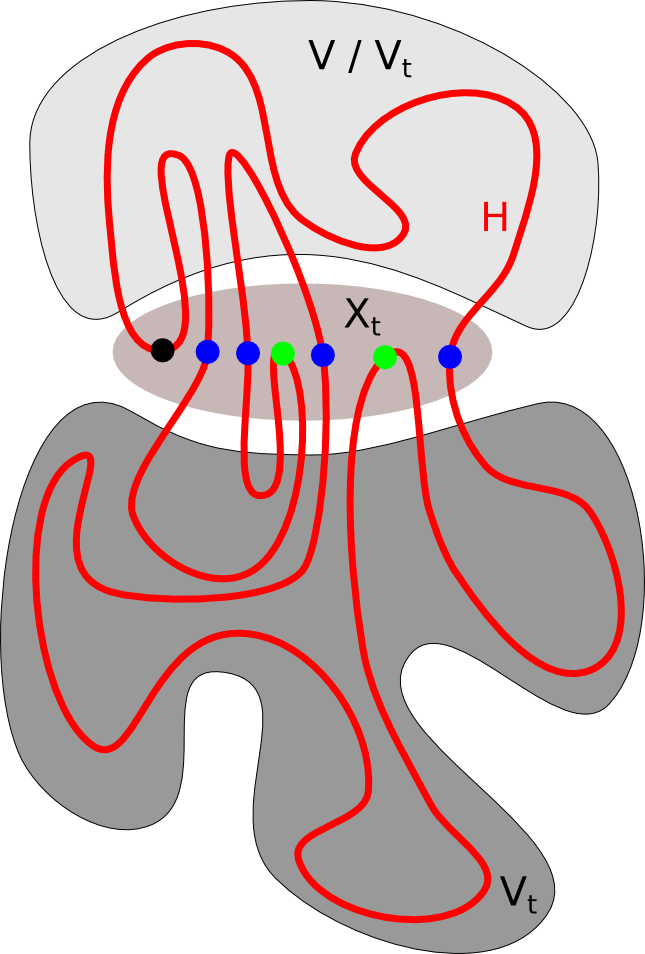
\includegraphics[scale=0.5]{src/figures/hcpd_hamilton_1.png}
        \caption{Représentation d'un cycle hamiltonien dans le graphe $G$ en fonction de $X_t$}
        \label{hcpd_h1}
    \end{center}
\end{figure}

\begin{figure}
    \begin{center}
        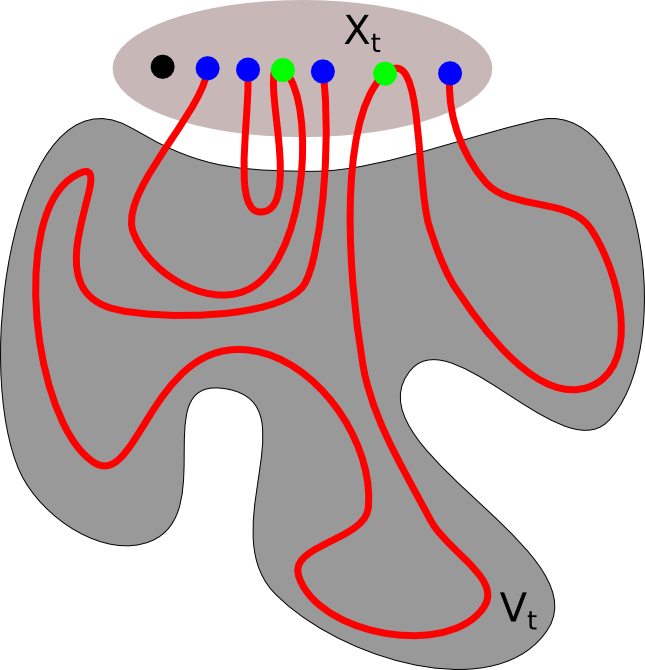
\includegraphics[scale=0.5]{src/figures/hcpd_hamilton_2.png}
        \caption{Représentation de la collection de chemins $H[V_t]$}
        \label{hcpd_h2}
    \end{center}
\end{figure}

\begin{figure}
    \begin{center}
        \hfill
        \subfloat[Collection $1$]{
            \label{fig:g1}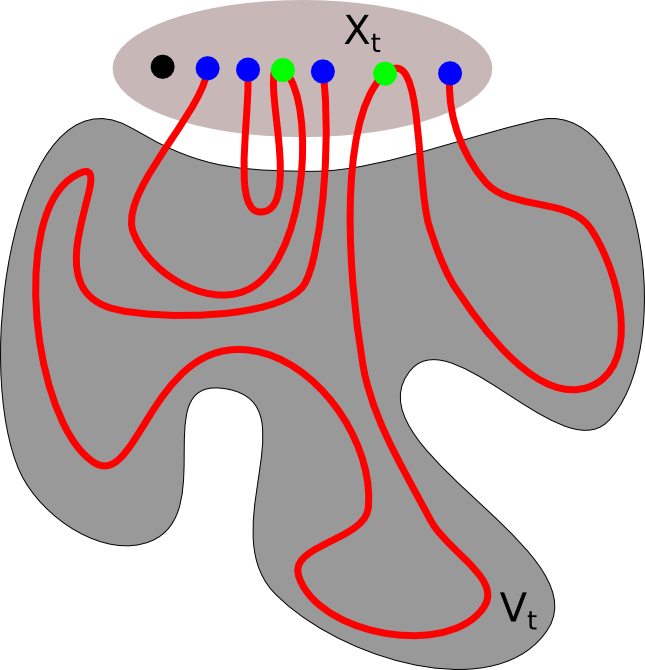
\includegraphics[scale=0.3]{src/figures/hcpd_hamilton_2.png}
        }
        \hfill
        \subfloat[Collection $2$]{
            \label{fig:g2}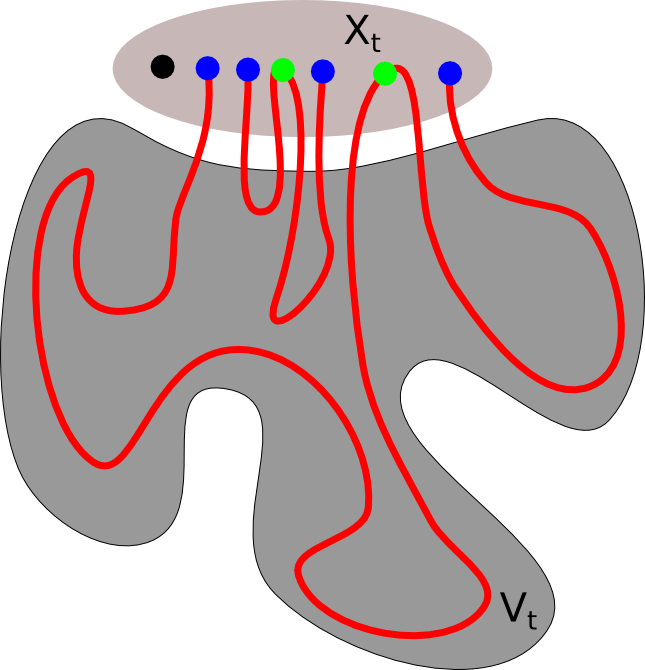
\includegraphics[scale=0.3]{src/figures/hcpd_hamilton_3g2.png}
        }
        \hfill
    \end{center}
    \caption{Deux collections de chemin différentes pour un même sac $X_t$}
    \label{hcpd_h3}
\end{figure}

\begin{figure}
    \begin{center}
        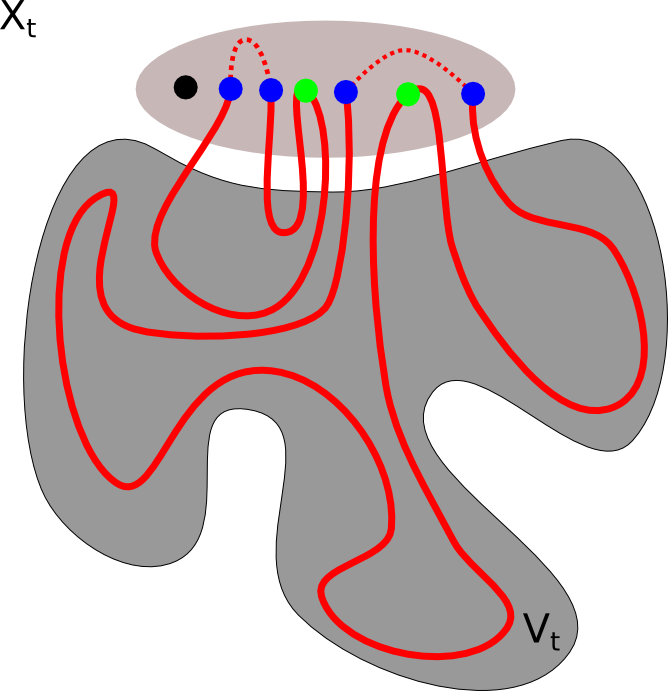
\includegraphics[scale=0.5]{src/figures/hcpd_hamilton_4.png}
        \caption{Représentation d'une solution partielle pour $X_t$}
        \label{hcpd_h1}
    \end{center}
\end{figure}

% }}}

%% }}}
%% {{{ ACTIONS SUR CHACUN DES NOEUDS
\section{La résolution du problème}

La question qui se pose à présent est de savoir comment calculer les solutions partielles d'un sac
$t \in T$. Il est possible de calculer ces solutions à partir des solutions des fils de $t$. C'est
ce que nous allons voir en étudiant les différents cas possibles.

\subsection{Le sac feuille}

Si $t$ est une feuille alors $X_t = \{x\}$ et $t$ n'a aucun fils. $x$ est donc obligatoirement de
degré $0$ et $(\{x\}, \emptyset, \emptyset, \emptyset)$ est une solution partielle.

\subsection{Le sac suppression}

$t$ est un sac suppression, il a donc un fils $t_f$ contenant $v$ tel que $X_{t_f} = X_t \cup
\{v\}$. 
\begin{nlemma}
    Soit $s_{t_f} = \pdsol{t_f}$ une solution partielle pour $t_f$ alors $s_t = (X_{t_f}^0, X_{t_f}^1,
    X_{t_f}^2\backslash\{v\}, M_{t_f})$ est une solution partielle pour $t$.
\end{nlemma}

\begin{proof}
    Remarquons de prime abord de $X_t$ est un séparateur de $G$ donc tout sommet $v$ n'appartenant
    pas à $X_t$ et appartenant à l'un des descendants $t'$ de $t$ est interne à $G_t$. Ainsi si $v$
    appartient à une solution partielle de $t_f$, alors $v \in X_{t_f}^2$. Le problème $\pdsol{t_f}$ pour
    $t_f$ est équivalent au problème $(X_t^0, X_t^1, X_t^2\backslash\{v\}, M_t)$ pour $t$, donc une
    solution partielle pour le problème pour $t$ existe si et seulement si le une solution partielle
    du problème pour $t_f$ existe.
\end{proof}

\subsection{Le sac ajout}

Si $t$ est un sac ajout, il a un fils $t_f$ et contient un sommet $v$ tel que $X_{t} = X_{t_f} \cup
\{v\}$.

Trois cas sont ici possibles, dépendant du degré du sommet $v$ rajouté.

\subsubsection{Le sommet $v$ appartient à $X_t^0$}

\begin{nlemma}
    $\pdsol{t_f}$ est une solution partielle pour $t_f$ si et seulement si $(X_{t_f}^0 \cup \{v\},
    X_{t_f}^1, X_{t_f}^2, M_{t_f})$ est une solution partielle pour $t$.
\end{nlemma}

La démonstration est évidente.

\subsubsection{Le sommet $v$ appartient à $X_t^1$}

\begin{nlemma}
    Il existe un sous problème $\pdsol{t_f}$ pour $t_f$ équivalent au sous problème $\pdsol{t}$ pour
    $t$.
\end{nlemma}

\begin{proof}
    Par définition du sac ajout, il existe un n\oe d $v$ appartenant à $X_t$ et pas à $X_{t_f}$,
    Puisque $X_{t_f}$ est un séparateur les voisins de $v$ appartiennent à $X_t$, or par hypothèse
    de départ, $v \in X_t^1$, donc $v$ a exactement un voisin $u$ dans $X_t$ et donc dans $X_{t_f}$.
    Décrivons deux cas :
    \begin{itemize}
        \item $u \in X_t^2$, dans ce cas $u \in X_{t_f}^1$ ce qui implique qu'il existe un sommet $w
            \in X_{t_f}^1$ tel que $(u,w) \in M_{t_f}$. On peut alors définir $M_t$ de la façon
            suivante : \[
                M_t = M_{t_f} \backslash \{(u,w)\} \cup \{(v,w)\}
            \]. C'est de cette façon que $u$ devient un n\oe ud interne dans $X_t$. Et donc le
            problème $\pdsol{t_f}$ est équivalent au sous problème $\pdsol{t}$ avec :
            \[
                \begin{array}{rcl}
                    X_t^0 & = & X_{t_f}^0 \\
                    X_t^1 & = & X_{t_f}^1 \backslash \{u\} \cup \{v\}\\
                    X_t^2 & = & X_{t_f}^2 \cup \{u\}\\
                \end{array}
            \]
        \item $u \in X_t^1$, dans ce cas, $u \in X_{t_f}^0$. Et donc le sous problème $\pdsol{t_f}$
            est équivalent au sous problème $\pdsol{t}$ avec :
            \[
                \begin{array}{rcl}
                    X_t^0 & = & X_{t_f}^0 \backslash \{u\} \\
                    X_t^1 & = & X_{t_f}^1 \cup \{u\}\\
                    X_t^2 & = & X_{t_f}^2\\
                    M_t = M_{t_f} \cup \{(u, v)\}\\
                \end{array}
            \]
    \end{itemize}
\end{proof}

\begin{ncorol}
    $\pdsol{f_t}$ est une solution partielle pour $t_f$, si et seulement si $(X_{t_f}^0, X_{t_f}^1
    \backslash \{u\} \cup \{v\},X_{t_f}^2 \cup \{u\},M_{t_f} \backslash \{(u,w)\} \cup \{(v,w)\})$
    et/ou $X_{t_f}^0 \backslash \{u\}, X_{t_f}^1 \cup \{u\}, X_{t_f}^2, M_{t_f} \cup \{(u, v)\})$ est
    une solution partielle pour $t$.
\end{ncorol}

\subsubsection{$v$ appartient à $X_t^2$}

\begin{nlemma}
    Il existe un sous problème $\pdsol{t_f}$ pour $t_f$ équivalent au sous problème $\pdsol{t}$ pour
    $t$.
\end{nlemma}

\begin{proof}
    Ce cas est très similaire au cas précédent à ceci près, $v$ est relié à deux sommets $u, w$ de
    $X_t$ pouvant chacun appartenir soit à $X_t^2$ (et dont à $X_{t_f}^1$) soit à $X_t^1$ (et donc à
    $X_{t_f}^0$).

    Détaillons donc les trois cas : \begin{enumerate}
        \item $u, w \in X_{t_f}^1$, dans ce cas $v$ relie $u$ et $w$ et il existe $k, l \in
            X_{t_f}^1$ tels que $(k, u), (l,w) \in M$. Il suffit donc d'enlever les
            couples $(k, u)$ et $(l,w)$ au couplage $M_{t_f}$ et de lui ajouter le couple $(k, l)$
            pour obtenir $M_t$.
        \item $u, w \in X_{t_f}^0$, dans ce cas encore, $v$ relie $u$ et $w$ faisant passer leur
            degré à $1$, on obtient donc $M_t$ en ajoutant le couple $(u,w)$ à $M_{t_f}$
        \item $u \in X_{f_t}^0$ et $w \in X_{f_t}^1$, dans ce cas, il existe $k \in X_{f_t}^1$ tel
            que le couple $(k,w) \in M_{t_f}$. Il suffit alors de supprimer $(k,w)$ à $M_{t_f}$ et
            de lui ajouter le couple $(k, u)$ pour obtenir $M$.
    \end{enumerate}
\end{proof}

\begin{ncorol}
    $\pdsol{f_t}$ est une solution partielle pour $t_f$ si et seulement si au moins l'une des trois
    propositions suivantes est une solution partielle pour $t$ :
    \begin{enumerate}
        \item $(X_{t_f}^0, X_{t_f}^1 \backslash \{u, w\}, X_{t_f}^2 \cup \{u, v, w\}, M \backslash
            \{(k, u), (l, w)\} \cup \{(k, l)\})$
        \item $(X_{t_f}^0 \backslash \{u, w\}, X_{t_f}^1 \cup \{u, w\}, X_{t_f}^2 \cup \{v\}, M \cup
            \{(u, w)\})$
        \item $(X_{t_f}^0 \backslash \{u\}, X_{t_f}^1 \backslash \{w\} \cup \{u\}, X_{t_f}^2 \cup
            \{v, w\}, M \backslash \{(k, w)\} \cup \{(k, u)\})$
    \end{enumerate}
\end{ncorol}
        
\subsubsection{Le sac fusion}

$t$ est un sac fusion il possède donc deux fils $t_1$ et $t_2$ tels que $X_t = X_{t_1} = X_{t_2}$.
L'opération à réaliser est alors un fusion des solutions de $t_1$ et $t_2$ tout en vérifiant la
validité des solutions obtenues.

\begin{nlemma}
    Le sous problème $\pdsol{t}$ associé à $t$ admet au moins une solution si et seulement si il
    existe deux sous problème $\pdsol{t_1}$ et $\pdsol{t_2}$ associés à $t_1$ et $t_2$ vérifiant les
    conditions suivantes :
    \begin{enumerate}
        \item $X_{t_1}^2 \subseteq X_{t_2}^0$ et $X_{t_1}^1 \subseteq X_{t_2}^1 \cup X_{t_2}^0$
        \item $X_{t_2}^2 \subseteq X_{t_1}^0$ et $X_{t_2}^1 \subseteq X_{t_1}^1 \cup X_{t_1}^0$
        \item $M_{t_1} \cup M_{t_2}$ ne contient pas de cycle
    \end{enumerate}
\end{nlemma}

%% }}}
% {{{ VALIDITE
% }}}
%% {{{ COMPLEXITE
%% }}}
% }}}


% !!!! A ne faire que si j'ai du temps en rabe
% {{{ D'AUTRES PROBLEMES
%% {{{ WEIGHTED INDEPENDANT SET
%% }}}
%% {{{ COLORATION
%% }}}
%% {{{ FEEDBACK VERTEX SET
%% }}}
% }}}

\chapter{Conclusion}
\label{open}
% {{{ OUVERTURE
%% {{{ BRANCHWIDTH
%% }}}
%% {{{ PATHWIDTH
%% }}}
%% {{{ MSOL
%% }}}
% }}}





\bibliographystyle{plain}
\bibliography{src/bib} 
\end{document}
